\documentclass[10pt]{article}
\usepackage{pdfpages}
\usepackage{enumitem}
\usepackage{multirow}

\title{\textbf{DASH} \\Documentation}
\date{January 22, 2015}
\author{Zachary Pierson}

\begin{document}
\maketitle

%push the table of contents to the bottom of the page
\newpage
\par\vspace{\fill}
\tableofcontents
\newpage

\section{Introduction}
\paragraph{}
The c program dash is a result of the Computer Science Course 456, Operating Systems. The purpose of assignment 1 is to familiarize ourselves with the proc filesystem. Each process has a unique process ID, pid, associated with the process. the kernel exports a significant amount of process information in the /proc directory. There you can see numerical directories, indicating running processes. You can see some examples by typing ps aux at the command prompt of the shell.

\subsection{Description of Program}
\subparagraph{}
dash is a process identification program. It allows the user to find process id's based on a command string, and find command strings based on process id's. dash is also capable of providing the user with process information.

Once invoked, dash will enter an event loop awaiting user input. Acceptable command options can be found in Table \ref{table:dashcmds} on page \pageref{table:dashcmds}.

\begin{table}[b]
\centering
\begin{tabular}{l|l}
	Command & Description\\\hline
	\textbf{cmdnm} & finds command string based on given pid\\
	\textbf{pid} & finds pid based on given command string\\
	\textbf{systat} & process information dump\\
	\textbf{help} & prints information on available commands\\
	\textbf{exit/quit} & exits the program\\
\end{tabular}
\caption{dash commands}
\label{table:dashcmds}
\end{table}

\subsection{Compiling Instructions}
\subparagraph{}
The file can be found on github at:  https://github.com/zjpierson/operatingSystems/prog1
The Makefile supplied in the git repository is set up to compile the program into an executable called dash. This can be achived simply by typing \texttt{make} on the command line. To compile using gcc on the command line:
\begin{center}
	\texttt{gcc -o dash dash.c cmdArgs.c}
\end{center}

\subsection{Using Dash}
\subparagraph{}
First you must run the executable. This will automatically start the dash command prompt. You will then be able to use the available commands as seen in Table \ref{table:dashcmds} on page \pageref{table:dashcmds} for information on processes.\\\\
\texttt{user@host\$ ./dash\\
		dash>}

\newpage

The \texttt{cmdnm} command has an optional \texttt{[pid]} argument for finding the command string. If no arguments are passed, dash will return a list of all command strings.  An example of it use is below.\\\\
\texttt
{
dash> cmdnm 1\\
systemd\\
dash> cmdnm\\
Please specify pid. Here is a list of all cmd names:\\
systemd\,\,\,\, kthreadd\,\,\,\,\,\, ksoftirqd/0\\
rcuos/0\,\,\,\, bioset\,\,\,\,\,\,\,\,\,\,\,\, ksmd\\
crond\,\,\,\,\,\,\,\,\, watchdog/3\, bash\\
dash
}\\

The \texttt{pid} command is practically a mirror image of the \texttt{cmdnm} command. It takes an optional command string argument \texttt{[cmdnm]} and returns a list of all pid's that has a matching substring with the \texttt{[cmdnm]} argument. If no arguments are passed, dash will retun a list of all process id's. An example of its use is below.\\\\
\texttt
{
dash> pid systemd\\
1\\
dash> pid\\
Please specify cmd name. Here is a list of all pid's:\\
1\,\,\,\, 2\,\,\,\, 3\,\,\,\, 5\\
7\,\,\,\, 8\,\,\,\, 9\,\,\,\, 10\\
11\,\,12\,\, 13\\
14
}\\

The \texttt{systat} command prints diagnostic information about the process. There is no argument call to this function. The following information is what \texttt{systat} will return:

\begin{enumerate}[noitemsep]
	\item Linux Version
	\item System Uptime
	\item Total Memory
	\item Free Memory
	\item CPU information
	\item Cache size
\end{enumerate}
\hfill

The \texttt{help} command displays usage information about the program and possible arguments for the command prompt. Finally the next two commands \texttt{quit} and \texttt{exit} terminates the program and can be used interchangeably. In fact they do \textbf{exactly} the same thing as they call the same function.
\newpage

\subsection{Libraries Used}
\subparagraph{}
\begin{table}[t]
\centering
\begin{tabular}{l|c}
	Libraries & Functions Used\\\hline\hline
	\multirow{2}{*}{$<$stdio.h$>$} 
		& \texttt{fopen(), fclose(), fscanf()}\\
	 & \texttt{printf(),fgets()}\\\hline
	\multirow{2}{*}{$<$string.h$>$}
	 & \texttt{strcpy(), strcat(), strcmp(), strch()}\\
		& \texttt{strspn(), strstr(), strtok(), strlen()}\\\hline
	$<$stdlib.h$>$ & \texttt{exit()}\\\hline
	$<$dirent.h$>$ & \texttt{opendir(), readdir(), closedir()}\\
\end{tabular}
\caption{Library Functions}
\label{table:libfuncs}
\end{table}

As Illustrated in Table \ref{table:libfuncs}, the included libraries provide the program with useful functions. The  \texttt{$<$stdio.h$>$} library provides standard input output functionality to communicate with the user. These functions are scattered everywhere within the program code.

The \texttt{$<$string.h$>$} library is used for string manipulation. This library has the most diverse use of its functions mainly because there is a lot of string parsing that happens within the proc filesystem in order to retrieve process information.

The \texttt{$<$stdlib.h$>$} library is included solely for one purpose; to allow the quit function to exit the dash process when called on the command prompt. This library is not essential because there are other ways to quit the program.

The \texttt{$<$dirent.h$>$} library is used to find all directory names within /proc. This is especially useful when the pid of a command string is unknown and we have to look in every process directory to find the matching command string.

\subsection{Program Structure}
\label{subsection:structure}
\subparagraph{}
The program is broken up into 3 separate files: dash.c, cmdArgs.c, and cmdArgs.h. A structure that is important to note is the array of function pointers declared externally in cmdArgs.h and defined in cmdArgs.c. That array is closely used with the commands array also defined externally in cmdArgs.h and defined in cmdArgs.c. These two arrays are used together in the event loop to call the approproate function. Section \ref{section:algorithms} will cover this more in depth. Below is the file structure.\\

\fbox{
	\begin{minipage}{17mm}
	\centering
	\begin{small}
	cmdArgs.c
	\end{small}
	\begin{scriptsize}
	quit()\\
	cmdnm()\\
	pid()\\
	systat()\\
	help()\\
	display()\\
	\end{scriptsize}
		\hfill\vspace{3mm}
	\end{minipage} 
	}
	\hspace{5mm}
\fbox{
	\begin{minipage}{17mm}
	\centering
	\begin{small}
	cmdArgs.h
	\end{small}
	\begin{scriptsize}
		libraries\\
		\#defines\\
		prototypes\\
	\end{scriptsize}	
		\hfill\vspace{10mm}
	\end{minipage} 
	}
	\hspace{5mm}
\fbox{
	\begin{minipage}{17mm}
	\centering
	\begin{small}
	dash.c
	\end{small}
	\begin{scriptsize}
	main()\\
	\end{scriptsize}
		\hfill\vspace{15mm}
	\end{minipage} 
	}

\section{Algorithms}
\label{section:algorithms}
\paragraph{}
As briefly mentioned in Section \ref{subsection:structure}, there is an array of function pointers used in the event loop to call the appropriate function. For modularity sake, the \texttt{\#define NUM\_CMDS} is used to keep track of the number of commands the user can enter. To add another command, one would simply increase \texttt{NUM\_CMDS} and add the function to both the \texttt{commands} array and the \texttt{func} array. Obviously the function would need to be declared in cmdArgs.h and defined in cmdArgs.c as well.

\subsection{Event Loop}
\subparagraph{}
As stated before in both Sections \ref{subsection:structure} \& \ref{section:algorithms}, the event loop makes use of function pointers to call the appropriate method. 


\subsection{Functions}
\subparagraph{}
This is a new Subsection of the Introduction

\subsubsection{cmdnm}
\subparagraph{}
This is a new Subsection of the Introduction

\subsubsection{pid}
\subparagraph{}
This is a new Subsection of the Introduction


\subsubsection{systat}
\subparagraph{}
This is a new Subsection of the Introduction


\subsubsection{exit}
\subparagraph{}
This is a new Subsection of the Introduction


\section{Testing and Verification}
\paragraph{}
Another section we will talk about will include a lot of interesting and promising things about our talk.

\subsection{Event Loop}
\subparagraph{}
This is a new Subsection of the Introduction

\subsection{cmdnm}
\subparagraph{}
This is a new Subsection of the Introduction

\subsection{pid}
\subparagraph{}
This is a new Subsection of the Introduction

\subsection{systat}
\subparagraph{}
This is a new Subsection of the Introduction

\subsection{exit}
\subparagraph{}
This is a new Subsection of the Introduction

\section{Description of Submission}
\paragraph{}
Another section we will talk about will include a lot of interesting and promising things about our talk.


\subsection{Another Subsection}
\subparagraph{}
A SUB PARAGRAPH!

\section{APPENDICES}
\appendix

\section{Program Assignment}
%\label{App:AppendixA}
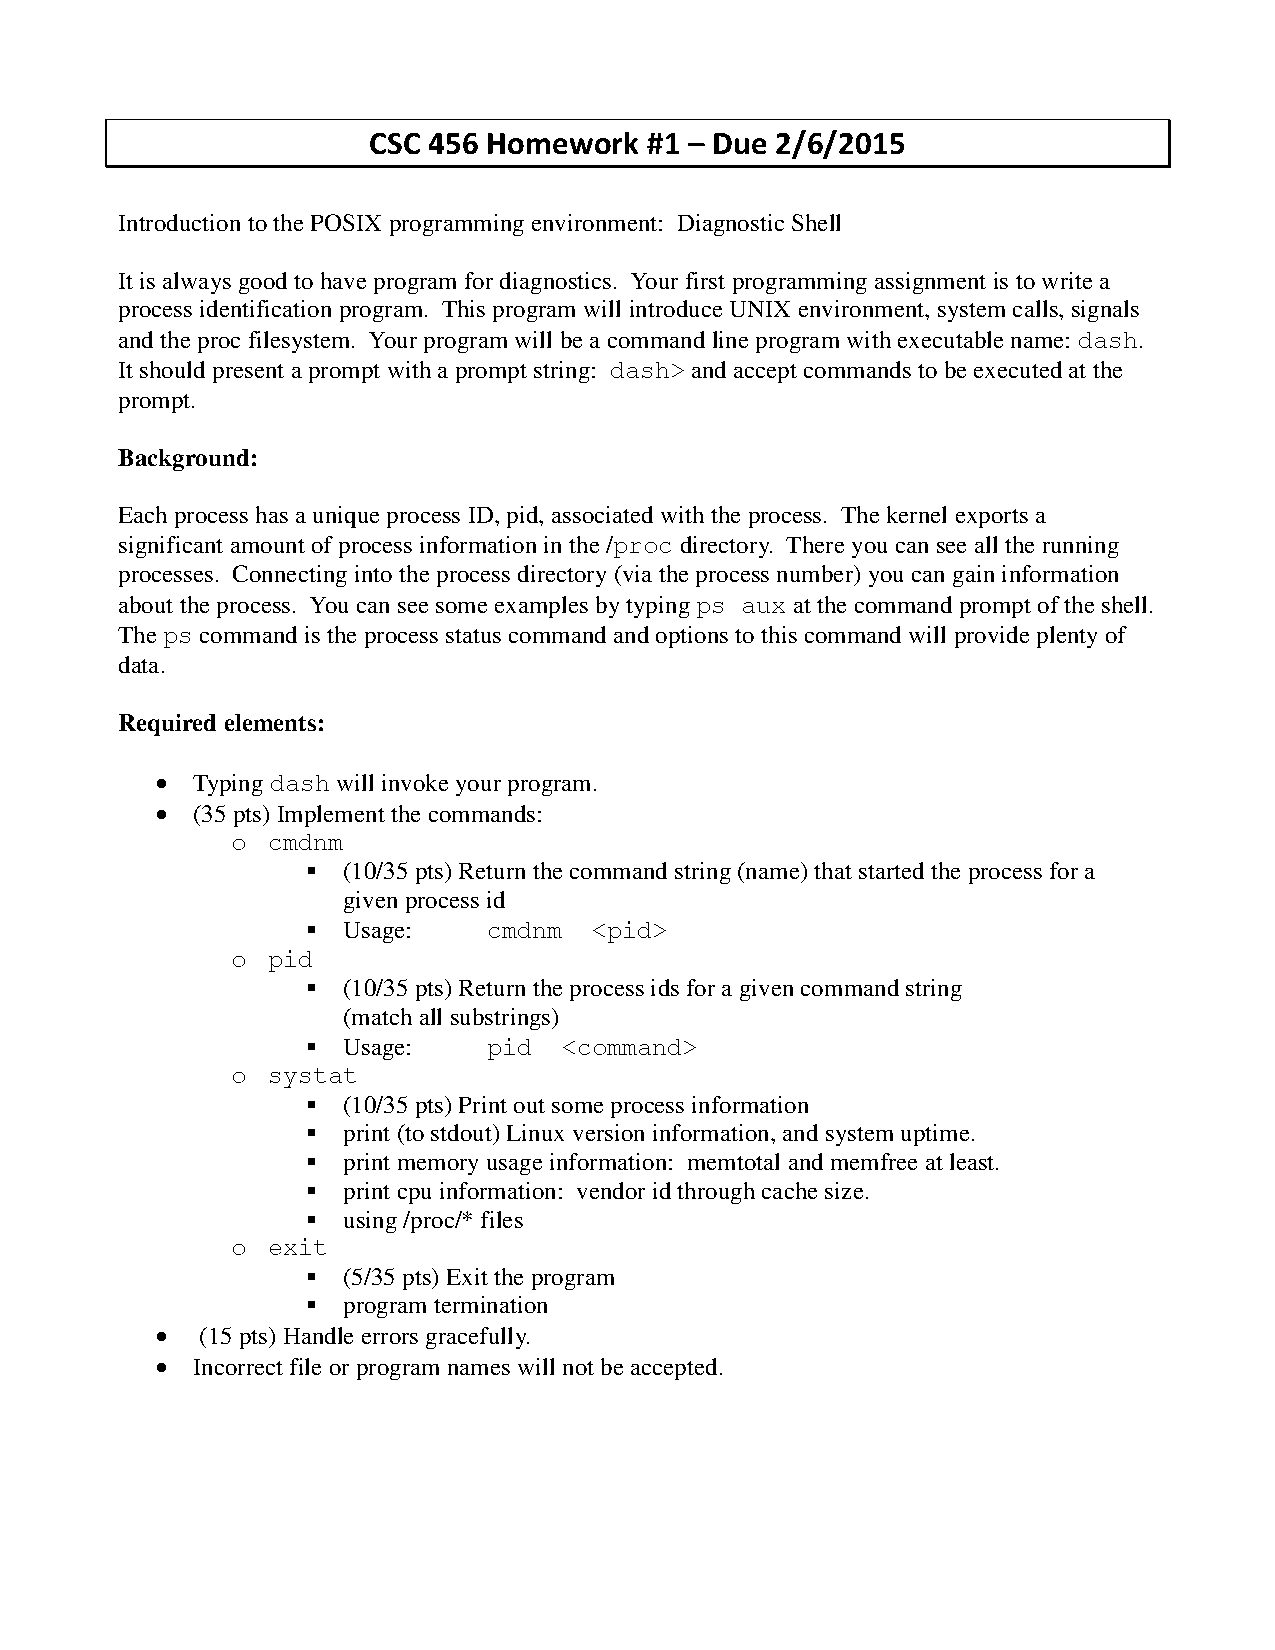
\includepdf[pages={1-4},frame={true}]{csc456_HW1.pdf}


\end{document}